\documentclass[11pt]{article}
\usepackage[toc,page]{appendix}
\usepackage{amsmath, amssymb}
\usepackage[utf8]{inputenc}
\usepackage[T1]{fontenc}
\usepackage[style=apa,backend=biber]{biblatex}
%\usepackage{biblatex}
\addbibresource{references.bib}
\usepackage{graphicx}
\usepackage{tikz}
\usetikzlibrary{automata,positioning,shapes.geometric, arrows.meta, fit, backgrounds, calc, chains}
\graphicspath{./images/Easy_Pictures/SMR_MULT_Repackaging}%\usepackage{kpfonts}
\usepackage{float}
\usepackage[margin=1in]{geometry}
\usepackage{cancel}
\usepackage{epsfig}
\usepackage{enumitem}
\usepackage{tikz-3dplot}
\usepackage{darkmode}
\usepackage{dirtytalk}
\usepackage{longtable,booktabs,array}
\usepackage{calc} % for calculating minipage widths
\usepackage[utf8]{inputenc}
\usepackage[T1]{fontenc}
\usepackage{xcolor}
\usepackage{listings}


\usepackage{etoolbox}
\usepackage{hyperref}
\hypersetup{
    colorlinks=true,
    linkcolor=blue,
    filecolor=magenta,      
    urlcolor=cyan,
    pdftitle={Hermeneutic Calculator},
    citecolor=blue,
    }


\urlstyle{same}

\lstdefinestyle{htmlStyle}{
    language=HTML,
    basicstyle=\ttfamily\small,
    keywordstyle=\color{blue}\bfseries,
    commentstyle=\color{gray}\itshape,
    stringstyle=\color{red},
    breaklines=true,
    frame=single,
    numbers=left,
    numberstyle=\tiny\color{gray},
    columns=fullflexible,
}
\lstdefinelanguage{HTML}{
  keywords={<!DOCTYPE, html, head, title, body, h1, h2, h3, p, div, span, a, img, ul, li, table, tr, td, th, style, link, script},
  sensitive=true,
  comment=[l]{//},
  morecomment=[s]{/*}{*/},
  morestring=[b]',
  morestring=[b]"
}
\lstset{style=htmlstyle, language=html}
% Updated to explicitly pass the language option
%\lstinputlisting[style=htmlstyle, language=html]{./html/example.html}
%\usepackage{tocloft}

% Optional: define some custom colors
\definecolor{sliceRed}{RGB}{225,224,91} % matching "varyellow" from your code
\definecolor{linkYellow}{RGB}{255,215,0}  % a golden yellow
\tdplotsetmaincoords{70}{110}

\title{Subtraction Strategies: Chunking}
\author{Compiled by: Theodore M. Savich}


\begin{document}
\maketitle



\subsection*{Transcript}
Video from \textcite{Carpenter1999}. Strategy descriptions and examples adapted from \textcite{HackenbergCourseNotes}. 


\begin{itemize}
    \item \textbf{Teacher:}``One summer T.J. saved \$400. At the end of the summer she spent \$294 on a new bike. How much money did T.J. have then?''
    \item \textbf{Student:} ``400 takeaway 200 is 200. I just put the 4 on the side right now. So then 200 takeaway 90 is 110. So then 110 takeaway 4 is 106. 
    \item \textbf{Teacher:} ``So how much money did she have left?''
    \item \textbf{Student:} ``106.''
    \item \textbf{Teacher:} ``Nice job.''
\end{itemize}

Here is the notation below to show what the student did:

\begin{align*}
400 - 200 &= 200\\
200 - 90 &= 110\\
110 - 4 &= 106
\end{align*}


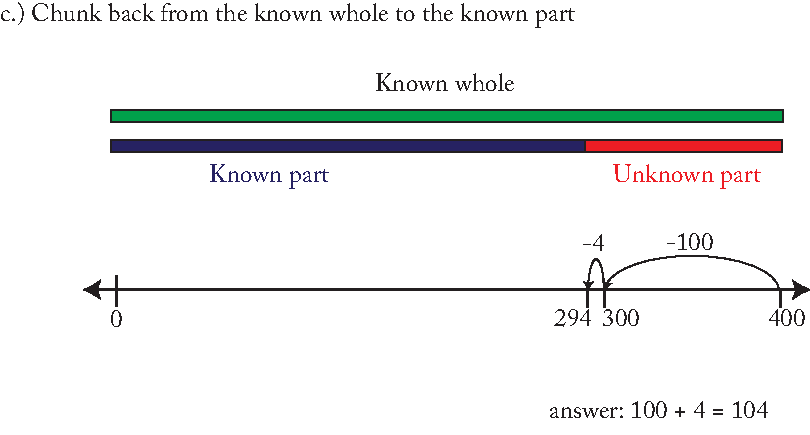
\includegraphics[width=.8\textwidth]{images/Easy_Pictures/SAR_SUB_CHUNKING_3_Ways/PDF/CHUNKING_BACKWARD_TO_KNOWN_PART.pdf}


However, this is only one of three structurally different ways that chunking can show up in subtraction. 

\begin{enumerate}[label=(\alph*)]
    \item \textbf{Chunking backwards (by known part)} The student starts at the known whole and subtracts backwards by the known part. They arrive at the unknown part. 
    \item \textbf{Chunking forwards} The student subtracts the known whole from the known part. 
    \item \textbf{Chunking backwards (to the known part)}  The student starts at the known whole and subtracts backwards until they reach the known part.
\end{enumerate}



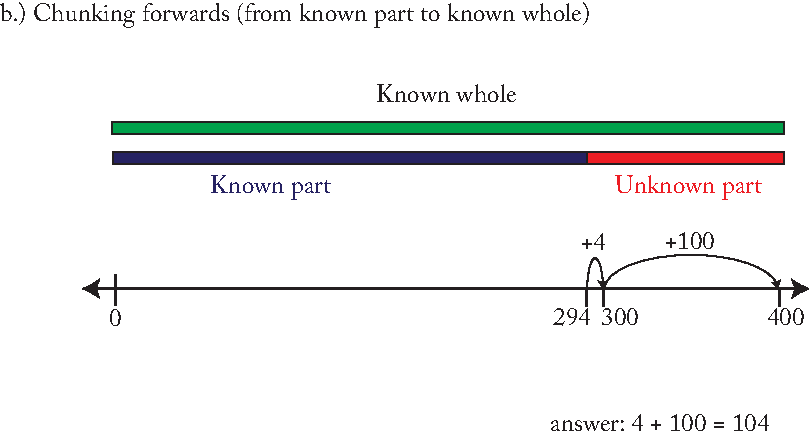
\includegraphics[width=.8\textwidth]{images/Easy_Pictures/SAR_SUB_CHUNKING_3_Ways/PDF/CHUNKING_FORWARD_FROM_KNOWN_PART.pdf}


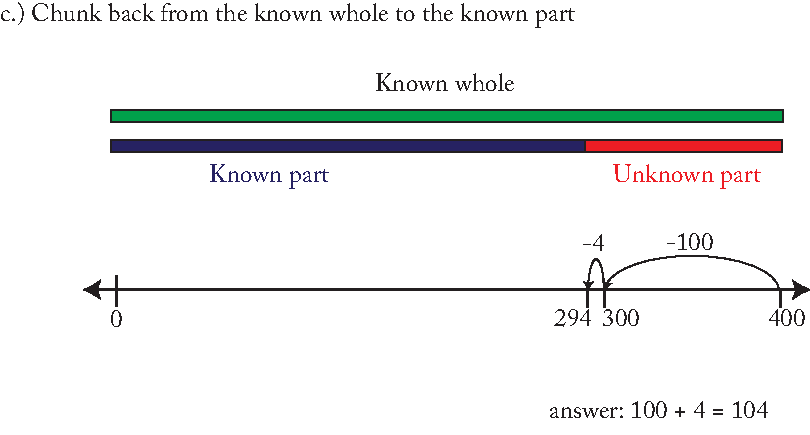
\includegraphics[width=.8\textwidth]{images/Easy_Pictures/SAR_SUB_CHUNKING_3_Ways/PDF/CHUNKING_BACKWARD_TO_KNOWN_PART.pdf}


\subsubsection*{Description of Strategy}
\begin{itemize}
    \item Subtract the subtrahend (known part) from the minuend (known whole) by breaking the subtrahend into bases and ones and subtracting in strategic chunks. 
    \item Start from the subtrahend and add strategic chunks to reach the minuend, summing the chunks to find the difference.
    \item Start at the minuend and subtract strategic chunks until you reach the subtrahend, summing the chunks to find the difference.
\end{itemize}

\subsubsection*{Automaton Type - only one type of chunking is analyzed here}
\textbf{Finite State Automaton (FSA) with Counters}:  
Counters are used to manage the sequential subtraction:
\begin{itemize}
    \item \textbf{BaseCounter:} Counts the number of base chunks to subtract.
    \item \textbf{OneCounter:} Counts the number of ones to subtract.
    \item \textbf{Difference:} Accumulates the running difference.
\end{itemize}

\subsubsection*{Formal Description of the Automaton}

We define the automaton as the tuple
\[
M = (Q,\, \Sigma,\, \delta,\, q_{0/accept},\, F,\, C)
\]
where:
\begin{itemize}
    \item \(Q = \{q_{0/accept},\, q_1,\, q_2,\, q_3\}\) is the set of states.
    \item \(\Sigma = \{0,1,2,3,4,5,6,7,8,9\}\) is the input alphabet (representing the digits of the minuend \(M\) and subtrahend \(S\)).
    \item \(q_{0/accept}\) is the start state, which is also the accept state.
    \item \(F = \{q_{0/accept}\}\) is the set of accepting states.
    \item \(C = \{\text{BaseCounter},\, \text{OneCounter},\, \text{Difference}\}\) is the set of counters.
\end{itemize}

The transition function \(\delta\) is defined as follows:
\begin{enumerate}
    \item \(\delta(q_{0/accept},\, \text{``}M,S\text{''}) = \) \\ \( (q_1,\, \text{initialize: set Difference} \gets M,\; \text{Decompose } S \text{ into BaseCounter and OneCounter})\).
    \item \(\delta(q_1,\, \varepsilon) = \) \\ \(  (q_2,\, \text{while BaseCounter} > 0:\; \text{Difference} \gets \text{Difference} - \text{(base chunk)},\; \text{decrement BaseCounter})\).
    \item \(\delta(q_2,\, \varepsilon) =  \) \\ \( (q_3,\, \text{when BaseCounter} = 0)\).
    \item \(\delta(q_3,\, \varepsilon) = \) \\ \(  (q_3,\, \text{while OneCounter} > 0:\; \text{Difference} \gets \text{Difference} - \text{(ones chunk)},\; \text{decrement OneCounter})\).
    \item \(\delta(q_3,\, \varepsilon) =  \) \\ \( (q_{0/accept},\, \text{when OneCounter} = 0:\; \text{output Difference})\).
\end{enumerate}

\subsubsection*{Automaton Diagram for Chunking by Bases and Ones (Forwards or Backwards)}

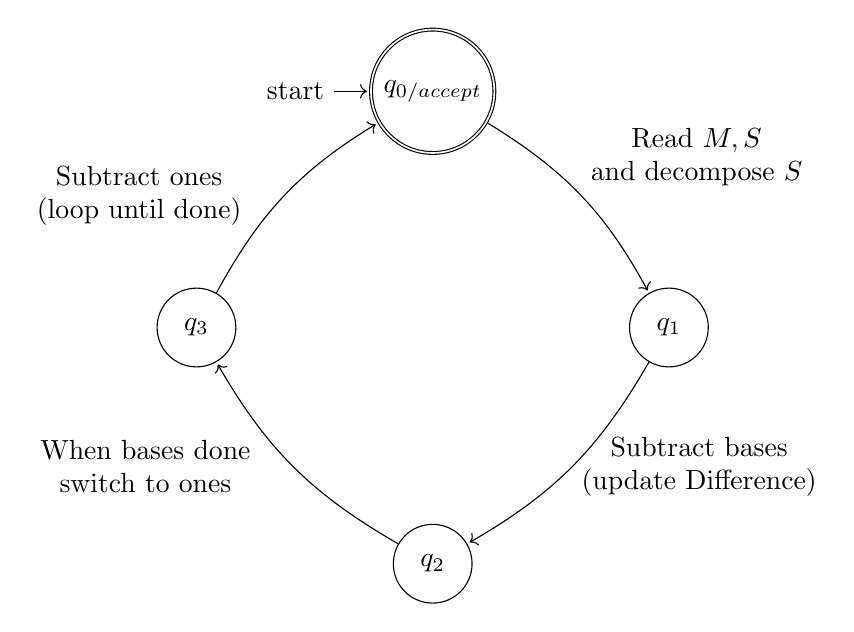
\begin{tikzpicture}[
    shorten >=1pt,
    auto,
    node distance=3cm,
    every state/.style={minimum size=1cm}
]
    % Arrange 4 states on a circle:
    \node[state, initial, accepting] (q0) at (90:3cm) {$q_{0/accept}$};
    \node[state] (q1) at (0:3cm) {$q_1$};
    \node[state] (q2) at (270:3cm) {$q_2$};
    \node[state] (q3) at (180:3cm) {$q_3$};
    
    \path[->]
        (q0) edge[bend left=15] node[above right, align=center] {Read \(M,S\)\\and decompose \(S\)} (q1)
        (q1) edge[bend left=15] node[right, align=center] {Subtract bases\\(update Difference)} (q2)
        (q2) edge[bend left=15] node[left=12pt, align=center] {When bases done\\switch to ones} (q3)
        (q3) edge[bend left=15] node[left=12 pt, align=center] {Subtract ones\\(loop until done)} (q0);
\end{tikzpicture}

\clearpage





\subsubsection*{HTML Implementation}
\lstinputlisting[style=htmlStyle, language=html]{./new_html/SAR_SUB_CHUNKING.html}

\printbibliography
\end{document}